\documentclass[11pt]{article}
\usepackage[scaled=0.92]{helvet}
\usepackage{geometry}
\geometry{letterpaper,tmargin=1in,bmargin=1in,lmargin=1in,rmargin=1in}
\usepackage[parfill]{parskip} % Activate to begin paragraphs with an empty line rather than an indent %\usepackage{graphicx}
\usepackage{amsmath,amssymb, mathrsfs, mathtools, dsfont}
\usepackage{tabularx}
\usepackage[font=footnotesize,labelfont=bf]{caption}
\usepackage{graphicx}
\usepackage{xcolor}
%\usepackage[linkbordercolor ={1 1 1} ]{hyperref}
%\usepackage[sf]{titlesec}
\usepackage{natbib}
\usepackage{../../Tianpei_Report}

%\usepackage{appendix}
%\usepackage{algorithm}
%\usepackage{algorithmic}

%\renewcommand{\algorithmicrequire}{\textbf{Input:}}
%\renewcommand{\algorithmicensure}{\textbf{Output:}}



\begin{document}
\title{Lecture 2: Smooth Maps}
\author{ Tianpei Xie}
\date{Oct. 14th., 2022}
\maketitle
\tableofcontents
\newpage
\section{Smooth Functions and Smooth Maps}
\subsection{Smooth Functions on Manifolds}
\begin{itemize}
\item 
\begin{definition}
Suppose $M$ is a smooth $n$-manifold, $k$ is a nonnegative integer, and $f: M \rightarrow \bR^k$ is any function. We say that $f$ is a \emph{\textbf{smooth function}} if for every $p \in M$, there exists a \emph{smooth chart} $(U, \varphi)$ for $M$ whose domain contains $p$ and such that the \emph{composite function} $f \circ \varphi^{-1}$ is smooth on the open subset $\widehat{U} = \varphi(U) \subseteq \bR^n$ (Fig. \ref{fig: smooth_fun}).

If $M$ is a smooth manifold \emph{with boundary}, the definition is exactly the same, except that $\varphi(U)$ is now an open subset of either 
$\bR^n$ or $\bH^n$, and in the latter case we interpret smoothness of $f \circ \varphi^{-1}$ to mean that each point of $\varphi(U)$ has a neighborhood (in $\bR^n$) on which $f \circ \varphi^{-1}$ \emph{extends to a smooth function} in the ordinary sense.
\end{definition}


\begin{figure}
\begin{minipage}[t]{1\linewidth}
  \centering
  \centerline{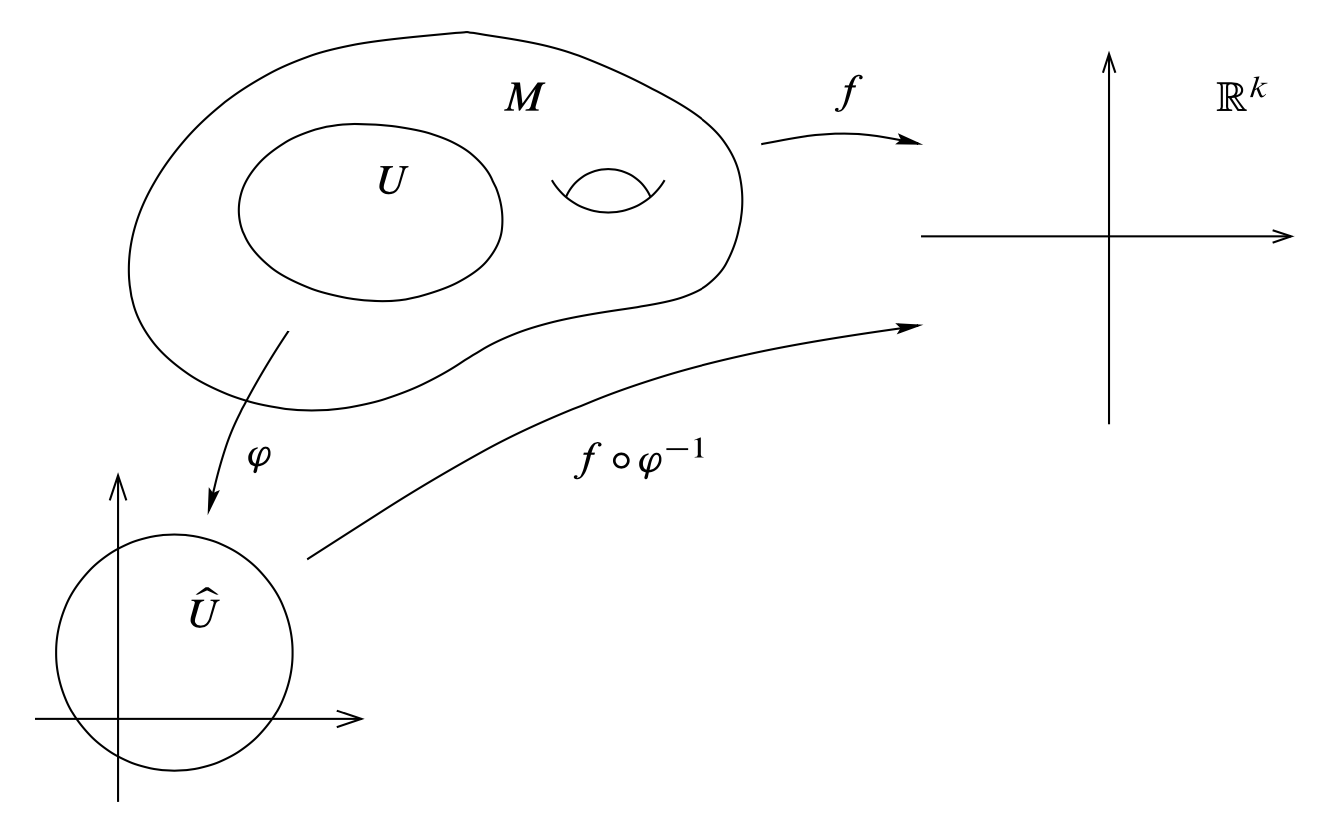
\includegraphics[scale = 0.5]{smooth_map.png}}
\end{minipage}
\caption{\footnotesize{\textbf{A smooth function on manifold \citep{lee2003introduction}}}}
\label{fig: smooth_fun}
\end{figure}

\item The most important special case is that of \emph{\textbf{smooth real-valued functions}} $f: M \rightarrow \bR$ the set of all such functions is denoted by $\cC^{\infty}(M)$. Because sums and constant multiples of smooth functions are smooth, $\cC^{\infty}(M)$ is a vector space over $\bR$.

\item \begin{definition}
Given a function $f: M \rightarrow \bR^k$ and a chart $(U, \varphi)$ for $M$, the function $\widehat{f}: \varphi(U) \rightarrow \bR^k$ defined by $\widehat{f}(x) = f \circ \varphi^{-1}(x)$ is called the \emph{\textbf{coordinate representation}} of $f$. 
\end{definition}

By definition, $f$ is \emph{smooth} \textbf{if and only} if its coordinate representation is \emph{smooth} in some smooth chart around \emph{each point}. \emph{Smooth functions have smooth coordinate representations in \textbf{every smooth chart}}.
\end{itemize}
\subsection{Smooth Maps Between Manifolds}
\begin{itemize}

\begin{figure}
\begin{minipage}[htb]{1\linewidth}
  \centering
  \centerline{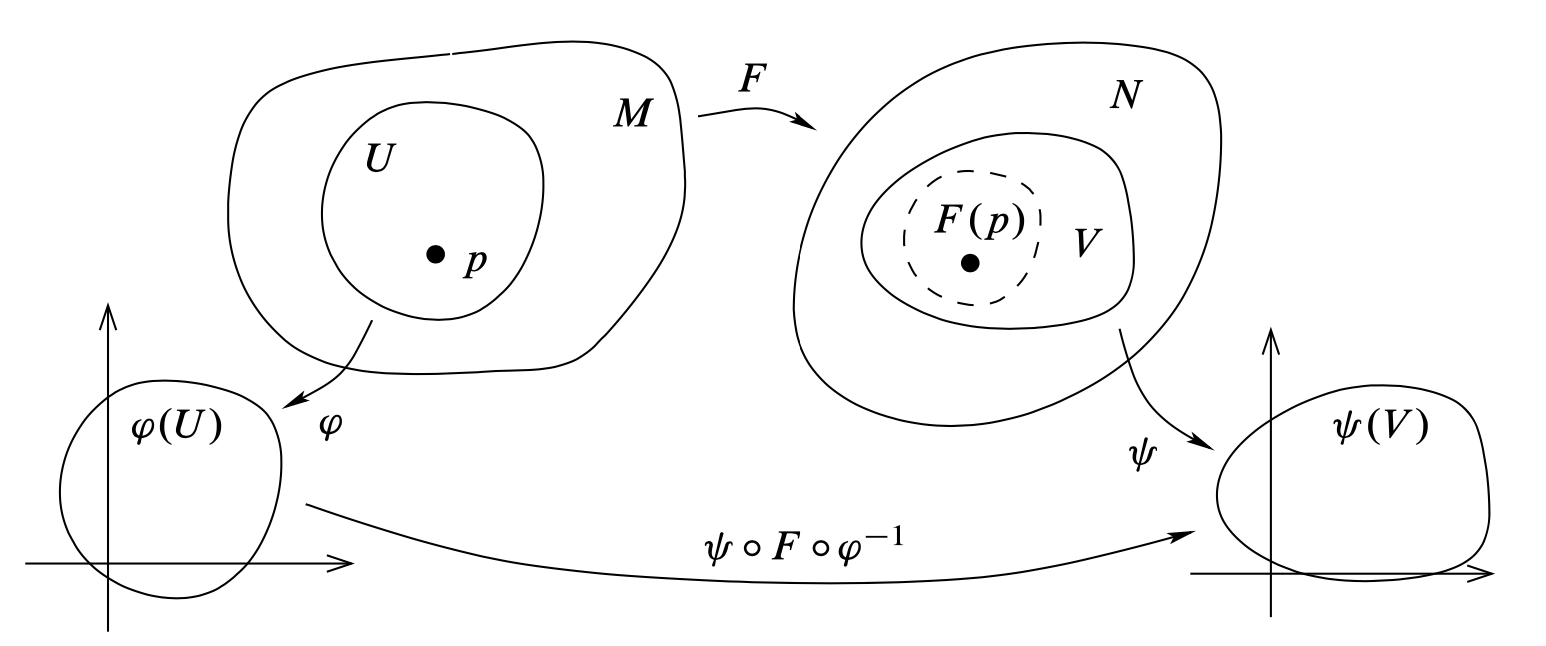
\includegraphics[scale = 0.5]{smooth_map_def.png}}
\end{minipage}
\caption{\footnotesize{\textbf{A smooth map between manifolds \citep{lee2003introduction}}}}
\label{fig: smooth_map}
\end{figure}

\item The definition of smooth functions generalizes easily to maps between manifolds.
\begin{definition}
Let $M, N$ be \emph{smooth manifolds}, and let $F: M \rightarrow N$ be any map. We say that $F$ is a \emph{\textbf{smooth map}} if for every $p \in M$, there exist \emph{smooth charts} $(U, \varphi)$ containing $p$ and $(V, \psi)$ containing $F(p)$ such that $F(U) \subseteq V$ and the composite map $\psi \circ F \circ \varphi^{-1}$ is \emph{\textbf{smooth}} from $\varphi(U)$ to $\psi(V)$. (See Fig. \ref{fig: smooth_map})

If $M$ and $N$ are smooth manifolds \emph{with boundary}, smoothness of $F$ is defined in exactly the same way, with the usual understanding that a map whose domain is a subset of $\bH^n$ is smooth if it admits an extension to a smooth map in a neighborhood of each point, and a map whose codomain is a subset of $\bH^n$ is smooth if it is smooth as a map into $\bR^n$.
\end{definition}

\item 
\begin{proposition}
Every smooth map is \textbf{continuous}.
\end{proposition}

\item 
\begin{proposition} (\textbf{Equivalent Characterizations of Smoothness}) \citep{lee2003introduction}\\
Suppose $M$ and $N$ are smooth manifolds with or without boundary, and $F: M \rightarrow N$ is a map. Then $F$ is \textbf{smooth} if and only if either of the following conditions is satisfied:
\begin{enumerate}
\item For every $p \in M$, there exist \textbf{smooth charts} $(U, \varphi)$ containing $p$ and $(V, \psi)$ containing $F(p)$ such that $U \cap F^{-1}(V)$ is \textbf{open} in $M$ and the composite map $\psi \circ F \circ \varphi^{-1}$ is \textbf{smooth} from $\varphi(U\cap F^{-1}(V))$ to $\psi(V)$.
\item $F$ is continuous and there exist \textbf{smooth atlases} $\set{(U_{\alpha}, \varphi_{\alpha})}$ and $\set{(V_{\beta}, \psi_{\beta})}$ for $M$ and $N$, respectively, such that for \textbf{each} $\alpha$ and $\beta$, $\psi_{\beta} \circ F \circ \varphi_{\alpha}^{-1}$ is a smooth map from $\varphi_{\alpha}(U_{\alpha}\cap F^{-1}(V_{\beta}))$ to $\psi_{\beta}(V_{\beta})$.
\end{enumerate}
\end{proposition}

\item
\begin{proposition} (\textbf{Smoothness Is Local}) \citep{lee2003introduction}\\
Let $M$ and $N$ be smooth manifolds with or without boundary, and let $F: M \rightarrow N$ be a map.
\begin{enumerate}
\item If every point $p \in M$ has a neighborhood $U$ such that the \textbf{restriction} $F|_{U}$ is smooth, then $F$ is smooth.
\item Conversely, if $F$ is smooth, then its restriction to \textbf{every open subset} is smooth.
\end{enumerate} 
\end{proposition}

\item \begin{corollary} (\textbf{Gluing Lemma for Smooth Maps}) \citep{lee2003introduction}\\
 Let $M$ and $N$ be smooth manifolds with or without boundary, and let $\set{U_{\alpha}}_{\alpha \in A}$ be an \textbf{open cover} of $M$. Suppose that for each $\alpha \in A$, we are given a smooth map $F_{\alpha}: U_{\alpha} \rightarrow N$ such that the maps agree on overlaps: $F_{\alpha}|_{U_{\alpha}\cap U_{\beta}} = F_{\beta}|_{U_{\alpha}\cap U_{\beta}}$ for all $\alpha$ and $\beta$. Then there exists a \textbf{unique smooth map} $F: M \rightarrow N$ such that $F|_{U_{\alpha}} = F_{\alpha}$, for each $\alpha \in A$.
\end{corollary}

\item 
\begin{definition}
If $F: M \rightarrow N$ is a \emph{smooth map}, and $(U, \varphi)$ and $(V, \psi)$ are any smooth charts for $M$ and $N$, respectively, we call $\widehat{F} = \psi \circ F \circ \varphi^{-1}$ the \emph{\textbf{coordinate representation}} of $F$ with respect to the given coordinates. It maps the set $\varphi(U\cap F^{-1}(V))$ to $\psi(V)$.
\end{definition}

\item 
\begin{proposition}
Let $M, N$ and $P$ be smooth manifolds with or without boundary.
\begin{enumerate}
\item Every \textbf{constant map} $c: M \rightarrow N$ is smooth.
\item The \textbf{identity map} of $M$ is smooth.
\item If $U \subseteq M$ is an \textbf{open submanifold} with or without boundary, then the \textbf{inclusion
map} $U \xhookrightarrow{} M$ is smooth.
\item If $F: M \rightarrow N$ and $G: N \rightarrow P$  are smooth, then so is the \textbf{composite map} $G \circ F: M \rightarrow P$.
\end{enumerate}
\end{proposition}

\item 
\begin{proposition}
Suppose $M_1 ,\ldots, M_k$ and $N$ are smooth manifolds with or without boundary, such that at most one of $M_1 ,\ldots, M_k$ has \textbf{nonempty boundary}. For each $i$, let $\pi_i: M_1 \times \ldots \times M_k \rightarrow M_i$ denote the \textbf{projection} onto the $M_i$ factor. A map $F: N \rightarrow M_1 \times \ldots \times M_k$ is smooth if and only if each of the \textbf{component maps} $F_i = \pi_i \circ F: N \rightarrow M_i$ is smooth.
\end{proposition}
\end{itemize}

\subsection{Examples of Smooth Map}
\begin{itemize}
\item \begin{example}
Any map from a zero-dimensional manifold into a smooth manifold with or without boundary is automatically smooth, because each coordinate representation is \textbf{constant}.
\end{example}

\item \begin{example}
If the \emph{circle} $\bS^1$ is given its \emph{standard smooth structure}, the map $\epsilon: \bR \rightarrow \bS^1$ defined by $\epsilon(t) = \exp\paren{2\pi i t}$ is \emph{smooth}, because with respect to any angle coordinate $\theta$ for $\bS^1$ it has a coordinate representation of the form $\widehat{\epsilon}(t) = 2 \pi t + c$ for some constant $c$, as you can check.
\end{example}

\item \begin{example}
The map $\epsilon^n: \bR^{n} \rightarrow \mathbb{T}^n$ defined by $\epsilon^n(t) = \paren{\exp\paren{2\pi i x^1}, \ldots, \exp\paren{2\pi i x^n}}$ is \emph{smooth} since \emph{$n$-torus} $\mathbb{T}^n = \bS\times \ldots \times \bS$.
\end{example}

\item \begin{example}
Now consider the $n$-sphere $\cS^n$ with its \emph{standard smooth structure}. The \textbf{\emph{inclusion map}} $\iota: \bS^n \xhookrightarrow{} \bR^{n+1}$ is certainly \emph{continuous}, because it is the inclusion map of a topological subspace. It is a smooth map because its coordinate representation with respect to any of the graph coordinates
\begin{align*}
\widehat{\iota} = \iota \circ (\varphi_{i}^{\pm})^{-1}(u^1, \ldots, u^n) =  \paren{u^1, \ldots, u^{i-1}, \sqrt{1 - \norm{u}{2}}, u^{i+1}, \ldots, u^{n}}
\end{align*} which is \emph{smooth} on its domain.
\end{example}

\item \begin{example}
The \emph{\textbf{quotient map}} $\pi: \bR^{n+1} \setminus \set{0} \rightarrow \bR\bP^n$ used to define $\bR\bP^n$ is \emph{smooth}, because its coordinate representation in terms of any of the coordinates for $\bR\bP^n$ constructed in Example before and standard coordinates on $\bR^{n+1} \setminus \set{0}$ is
\begin{align*}
\widehat{\pi}(x^1, \ldots, x^{n+1}) &= \varphi_{i} \circ \pi(x^1, \ldots, x^{n+1}) =\varphi_{i}[x^1, \ldots, x^{n+1}] \\
&= \paren{\frac{x^1}{x^{i}}, \ldots, \frac{x^{i-1}}{x^{i}}, \frac{x^{i+1}}{x^{i}},\ldots, \frac{x^{n+1}}{x^{i}}}.
\end{align*}
\end{example}

\item \begin{example}
Define $q: \bS^n \rightarrow \bR\bP^n$ as the restriction of $\pi: \bR^{n+1} \setminus \set{0} \rightarrow \bR\bP^n$ to $\bS^n \subseteq  \bR^{n+1} \setminus \set{0}$. It is a \emph{smooth} map, because it is the composition $q = \pi \circ \iota$ of the maps in the preceding two examples.
\end{example}

\item \begin{example}
If $M_1 ,\ldots, M_k$ are smooth manifolds, then each projection map $\pi_i: M_1 \times \ldots \times M_k \rightarrow M_i$ is \emph{smooth}, because its coordinate representation with respect to any of the product charts of Example 1.8 is just a coordinate projection.
\end{example}

\end{itemize}

\subsection{Diffeomorphisms}
\begin{itemize}
\item \begin{definition}
If $M$ and $N$ are smooth manifolds with or without boundary, a \emph{\textbf{diffeomorphism}} from $M$ to $N$ is a \emph{\textbf{smooth bijective map}} $F: M \rightarrow N$ that has a \emph{\textbf{smooth inverse}}. We say that $M$ and $N$ are \emph{\textbf{diffeomorphic}} if there exists a \emph{diffeomorphism} between them. Sometimes this is symbolized by $M \approx N$.
\end{definition}

\item \begin{example}
If $M$ is any smooth manifold and $(U, \varphi)$ is a smooth coordinate chart on $M$, then $\varphi: U \rightarrow \varphi(U) \subseteq \bR^n$ is a \emph{\textbf{diffeomorphism}}. (In fact, it has an identity map as a coordinate representation.)
\end{example}

\item \begin{proposition} (\textbf{Properties of Diffeomorphisms})
\begin{enumerate}
\item Every \textbf{composition} of diffeomorphisms is a diffeomorphism.
\item Every \textbf{finite product} of diffeomorphisms between smooth manifolds is a diffeomorphism.
\item Every diffeomorphism is a \textbf{homeomorphism} and an \textbf{open map}.
\item The \textbf{restriction} of a diffeomorphism to an open submanifold with or without boundary is a diffeomorphism onto its image.
\item "Diffeomorphic" is an \textbf{equivalence relation} on the class of all smooth manifolds.
with or without boundary.
\end{enumerate}
\end{proposition}

\item The following theorem is a weak version of \emph{invariance of dimension}, which suffices for many purposes.
\begin{theorem} (\textbf{Diffeomorphism Invariance of Dimension}).\\
A nonempty smooth manifold of dimension $m$ cannot be diffeomorphic to an $n$-dimensional smooth manifold unless $m = n$.
\end{theorem}

\item \begin{theorem} (\textbf{Diffeomorphism Invariance of the Boundary}). \\
Suppose $M$ and $N$ are smooth manifolds with boundary and $F: M \rightarrow N$ is a diffeomorphism. Then $F(\partial\,M) = \partial\,N$, and $F$ restricts to a diffeomorphism from $\text{Int}\,M$ to $\text{Int}\,N$.
\end{theorem}

\item Just as two topological spaces are considered to be "the same" if they are \emph{\textbf{homeomorphic}}, two smooth manifolds with or without boundary are essentially indistinguishable if they are \emph{\textbf{diffeomorphic}}.

\item The \emph{\textbf{central concern}} of smooth manifold theory is the study of properties of smooth manifolds that are \emph{\textbf{preserved by diffeomorphisms}}. (This includes properties that are invariant under change of variables since the coordination itself is a diffemorphism. )

\item It is natural to wonder whether the smooth structure on a given topological manifold is \emph{unique}. This straightforward version of the question is easy to answer: we observed in Example before that every zero-dimensional manifold has a unique smooth structure, but each positive-dimensional manifold admits \emph{\textbf{many distinct smooth structures}} \emph{as soon as it admits one}.
\end{itemize}

\section{Partitions of Unity}
\subsection{Theorems}
\begin{itemize}
\item Recall the gluing lemma in topology
\begin{lemma}(\textbf{Gluing Lemma for Continuous Maps}). \\
Let $X$ and $Y$ be topological spaces, and suppose one of the following conditions holds:
\begin{enumerate}
\item  $B_1 \xdotx{,} B_n$ are \textbf{finitely} many \textbf{closed} subsets of $X$ whose union is $X$.
\item  $\set{B_i}_{i\in A}$ is a collection of \textbf{open} subsets of $X$ whose union is X.
\end{enumerate}
Suppose that for all $i$ we are given \textbf{continuous} maps $F_i: B_i \rightarrow Y$ that \textbf{agree on overlaps}: $F_i|_{B_i \cap B_j} = F_j|_{B_i \cap B_j}$. Then there exists a \textbf{unique continuous map} $F: X \rightarrow Y$ whose restriction to each $B_i$ is equal to $F_i$.
\end{lemma}

Comparing with the Gluing Lemma for smooth maps, we see that it does not hold for \emph{the finitely many \textbf{closed} subsets case}.
 \begin{corollary} (\textbf{Gluing Lemma for Smooth Maps}) \citep{lee2003introduction}\\
 Let $M$ and $N$ be smooth manifolds with or without boundary, and let $\set{U_{\alpha}}_{\alpha \in A}$ be an \textbf{open cover} of $M$. Suppose that for each $\alpha \in A$, we are given a smooth map $F_{\alpha}: U_{\alpha} \rightarrow N$ such that the maps agree on overlaps: $F_{\alpha}|_{U_{\alpha}\cap U_{\beta}} = F_{\beta}|_{U_{\alpha}\cap U_{\beta}}$ for all $\alpha$ and $\beta$. Then there exists a \textbf{unique smooth map} $F: M \rightarrow N$ such that $F|_{U_{\alpha}} = F_{\alpha}$, for each $\alpha \in A$.
\end{corollary}

\item 
\begin{remark}
A \emph{\textbf{disadvantage}} of Corollary above is that in order to use it, we must construct maps that agree exactly on relatively large subsets of the manifold, which is \emph{\textbf{too restrictive}} or some purposes. In this section we introduce \emph{\textbf{partitions of unity}}, which are tools for ``blending together" local smooth objects into global ones \emph{\textbf{without necessarily assuming that they agree on overlaps}}. 
\end{remark}

\item \begin{lemma}
The function $f: \bR \rightarrow \bR$ defined by
\begin{align*}
f(t) &= \left\{\begin{array}{cc}
e^{-1/t} & t > 0 \\
0 & t\le 0
\end{array} \right.
\end{align*} is \textbf{smooth}.
\end{lemma}

\item \begin{lemma}
Given any real numbers $r_1$ and $r_2$ such that $r_1 < r_2$, there exists a \textbf{smooth} function $h: \bR \rightarrow \bR$ such that $h(t) \equiv 1$ for $t \le r_1$, $0 < h(t) < 1$ for $r_1 < t < r_2$, and $h(t) = 0$ for $t >  r_2$.
\end{lemma} 

A function with the properties of $h$ in the preceding lemma is usually called \emph{\textbf{a cutoff function}}. Let $h = f(r_2 - t)/(f(r_2 -t ) + f(t - r_1))$ where $f$ is define in preivous lemma.

\item \begin{lemma}
Given any positive real numbers $r_1 < r_2$, there is a smooth function $H: \bR^n \rightarrow \bR$ such that $H \equiv 1$ on $\bar{B}_{r_1}(0)$,  $0 < H(x) < 1$ for all $x \in B_{r_2}(0) \setminus \bar{B}_{r_1}(0)$, and $H = 0$ on $\bR^n \setminus B_{r_2}(0)$.
\end{lemma} Let $H(x) = h(\norm{x}{})$ where $h$ is the cutoff function as above.

\item \begin{definition}
The function $H$ constructed in this lemma is an example of \emph{\textbf{a smooth bump function}}, a smooth real-valued function that is \emph{\textbf{equal to 1}} on a \emph{\textbf{specified set}} and is \emph{\textbf{zero outside a specified neighborhood}} of that set.
\end{definition}

\item \begin{definition}
If $f$ is any real-valued or vector-valued function on a topological space $M$, \emph{\textbf{the support of $f$}}, denoted by $\text{supp }f$, is the \emph{\textbf{closure}} of the set of points where $f$ is \emph{\textbf{nonzero}}:
\begin{align*}
\text{supp }f &= \overline{\set{p \in M: f(p) \neq 0}}
\end{align*} (For example, if H is the function constructed in the preceding lemma, then $\text{supp }H = \bar{B}_{r_2}(0)$.) If $\text{supp }f$ is contained in some set $U \subseteq M$, we say that \emph{\textbf{$f$ is supported in $U$}}. A function $f$ is said to be \emph{\textbf{compactly supported}} if $\text{supp }f$ is a \emph{compact set}. Clearly, every function \emph{on a compact space} is \emph{compactly supported}.
\end{definition}

\item \begin{definition}
Suppose $M$ is a topological space, and let $\cX = (X_{\alpha})_{\alpha \in A}$ be an arbitrary \emph{\textbf{open cover of $M$}}, indexed by a set $A$. \underline{\emph{\textbf{A partition of unity subordinate to $\cX$}}} is an indexed family $(\psi_{\alpha})_{\alpha \in A}$ of \emph{\textbf{continuous functions}} $\psi: M \rightarrow \bR$ with the following properties:
\begin{enumerate}
\item $0\le \psi_{\alpha}(x) \le 1$ for all $\alpha \in A$ and all $x \in M$.
\item \underline{$\text{supp }\psi_{\alpha} \subseteq X_{\alpha}$} for each $\alpha \in A$.
\item The family of supports $(\text{supp }\psi_{\alpha})_{\alpha \in A}$ is \underline{\emph{\textbf{locally finite}}}, meaning that every point has a \emph{neighborhood} that \emph{intersects} $\text{supp }\psi_{\alpha}$ for \emph{\textbf{only finitely many values}} of $\alpha$.
\item \underline{$\sum_{\alpha \in A}\psi_{\alpha}(x) = 1$} for all $x \in M$.
\end{enumerate}

If $M$ is a smooth manifold with or without boundary, \emph{\textbf{a smooth partition of unity}} is one for which each of the functions $\psi_{\alpha}$ is \emph{\textbf{smooth}}.
\end{definition}

\item \begin{theorem} (\textbf{Existence of Partitions of Unity}). \citep{lee2003introduction} \\
Suppose $M$ is a smooth manifold with or without boundary, and $\cX = (X_{\alpha})_{\alpha \in A}$ is any indexed \textbf{open cover} of $M$.
Then there \textbf{exists} a \textbf{smooth partition of unity} subordinate to $\cX$.
\end{theorem}
\end{itemize}
\subsection{Applications of Partitions of Unity}
\begin{itemize}
\item \begin{definition}
If $M$ is a topological space, $A \subseteq M$ is a \textbf{\emph{closed}} subset, and $U \subseteq M$ is an \textbf{\emph{open}} subset containing $A$, a \emph{\textbf{continuous}} function $\psi: M \rightarrow \bR$ is called \emph{\textbf{\underline{a bump function} for $A$ supported in $U$}} if $0\le \psi \le 1$ on $M$, $\psi \equiv
1$ on $A$, and $\text{supp }\psi \subseteq U$.
\end{definition}

\item \begin{proposition} (\textbf{Existence of Smooth Bump Functions}).   \citep{lee2003introduction}\\
Let $M$ be a smooth manifold with or without boundary. For any \textbf{closed} subset $A\subseteq M$ and any \textbf{open} subset $U$ containing $A$, there \textbf{exists} a \textbf{smooth bump function for $A$ supported in $U$}.
\end{proposition}

\item \begin{definition}
Suppose $M$ and $N$ are smooth manifolds with or without boundary, and $A \subseteq M$ is an arbitrary subset. We say that a map $F:A \rightarrow N$ is \emph{\textbf{smooth on $A$}} if it has a \emph{\textbf{smooth extension}} \emph{in a neighborhood of each point}: that is, if for every $p \in A$ there is \emph{an open subset} $W \subseteq M$ containing $p$ and \emph{\textbf{a smooth map}} $\widetilde{F}: W \rightarrow N$ whose \emph{\textbf{restriction} to $W \cap A$ \textbf{agrees} with $F$} .
\end{definition}

\item \begin{lemma} (\textbf{Extension Lemma for Smooth Functions}).  \citep{lee2003introduction} \\
Suppose $M$ is a smooth manifold with or without boundary, $A \subseteq M$ is a \textbf{closed} subset, and $f: A \rightarrow \bR^k$ is a
\textbf{smooth} function. For any open subset $U$ containing $A$, there exists a smooth function $\widetilde{f}: M \rightarrow \bR^k$ such that $\widetilde{f}|_{A} = f$ and $\text{supp }\widetilde{f} \subseteq U$.
\end{lemma}

\item \begin{definition} 
If $M$ is a topological space, \emph{\textbf{an exhaustion function}} for $M$ is a \emph{continuous function} $f: M \rightarrow \bR$ with the property that the set $f^{-1}((-\infty, c])$ (called \emph{\textbf{a sublevel set of $f$}} ) is \emph{\textbf{compact}} for each $c \in \bR$. 
\end{definition}
Example of exhaustion function
\begin{align*}
f(x) = \norm{x}{}^2, \quad f(x) = \frac{1}{1- \norm{x}{2}^2}
\end{align*}

\item \begin{proposition} (\textbf{Existence of Smooth Exhaustion Functions}).   \citep{lee2003introduction}\\
Every smooth manifold with or without boundary admits a \textbf{smooth positive exhaustion function}.
\end{proposition}

\item \begin{theorem} (\textbf{Level Sets of Smooth Functions}).  \citep{lee2003introduction}\\
 Let $M$ be a smooth manifold. If $K$ is any \textbf{closed subset} of $M$, there is a \textbf{smooth nonnegative function} $f: M \rightarrow \bR$
such that $f^{-1}(0) =  K$.
\end{theorem}
\end{itemize}
\newpage
\bibliographystyle{plainnat}
\bibliography{book_reference.bib}
\end{document}